\documentclass[a4paper,10pt]{report}
\usepackage{mathalpha}
\usepackage[utf8]{inputenc}
\usepackage{cancel}
\usepackage[margin=2cm]{geometry}
\usepackage{amsmath}
\usepackage{amssymb}
\usepackage{graphicx}

\graphicspath{ {./} }

% Title Page
\title{Mathematical methods}
\author{Lachlan Takumi Ikeguchi}

\begin{document}
\maketitle
\tableofcontents

\begin{abstract}
	This document was written to be used as a summary to help revise the content covered mathematical methods.  For any inquiries, feedback, and further explanations, contact lachlanprivate@duck.com or through the discord server: https://discord.gg/6P8rddkXFr
\end{abstract}

\section{Important symbols}
\begin{center}
	\begin{tabular}{l|lp{6cm}}
		Symbol & Mathematical definition          & Simple definition                               \\ \hline
		$\cup$ & $P(A \cup B) = P(A) + P(B)$      & Probability of A occuring \emph{or} B occuring  \\
		$\cap$ & $P(A \cap B) = P(A) \times P(B)$ & Probability of A occuring \emph{and} B occuring \\
	\end{tabular}
\end{center}

\pagebreak

\section{Arithmetic sequence}
An arithmetic sequence is a sequence of numbers where the terms are increasing or decreasing at a constant rate.  The recursive definition of a sequence is:
$$t_{n + 1} = t_n + d$$
where $t_{n + 1}$ is the next term, $t_n$ is the current term, and $d$ is the common difference or ``by how much the sequence goes up by"\\

And the general equation for finding the $n^{\text{th}}$ term of the sequence is:
$$t_n = t_1 + (n - 1)d$$
$t_n$ is the $n^{\text{th}}$ term of the sequence, $t_1$ is the first term of the sequence, and $d$ is the common difference.

\subsection{Sum of all prior arithmetic sequence}
The sum of all arithmetic sequence is given by:
$$S_n = \frac{n}{2}(2t_1 + (n - 1)d) = \frac{n}{2}(t_1 + t_n)$$

\section{Functions}
Functions is an mathematical concept where if given an input, it performs some operations, and returns an output.  They have the mathematical notation of $f(x)$ where $f$ can be seen as the name of the function and the values within the parenthesis as inputs to the function.  A function must be defined for it to be used.  A simple function which calculates the y-values along a parabola with the x-coordinates as input could be:
$$M(x) = x^2$$

This function would return the values:
\begin{center}
	\begin{tabular}{l|l}
		$x$ & $M(x)$ \\ \hline
		-3  & 9      \\
		-2  & 4      \\
		-1  & 1      \\
		0   & 0      \\
		1   & 1      \\
		2   & 4      \\
		3   & 9
	\end{tabular}
\end{center}

Functions can only give an one-to-one relation or a many-to-one relation since there is a clear defined input and output values with the concept of a function.  To check if a graph is a function a \emph{vertical line test} can be performed:\\

If the graph intersects any vertical line more than once, it cannot be a function, and is instead a relation.

\section{Interval notation}
Interval notation are used to define the range of a function or a relation.  For example, if given a function where the y-values start at 0 and approach but never reach 1, to define the range of the function, it would be $0 \leq y < 1$.  However, this can be rewritten using interval notation as: [0, 1).  The square bracket meaning that it is equal to and less than or greater than, and the parenthesis meaning that it is greater than or less than but never reaching the value.\\

\begin{center}
	\emph{NOTE:  it is called a ``range" when it is the y-value, and a ``domain" when it is the x-value}
\end{center}

\section{Relations and Functions}
There are four types of relations, relations meaning for any x-value, how many valid y-values there are.  The four are: one-to-one, many-to-one, one-to-many, and many-to-many.\\

The first, (one-to-one) relation means that for any x-values, there is only one y-value.  An example would be a straight line: $f(x) = 2x + 3$.  The second, (many-to-one) relation means that for any y-values, there are more than one x-value.  An example would be a parabola: $f(x) = x^2$.  The previous are examples of functions, the next two are not.  The third, (one-to-many) relations means that for any x-value, there are more than one y-value.  And for the last, (many-to-many) relations means that for any x-value, there are more than one y-value, and the reverse is also true.

\section{Transformations}
The ways a function can be transformed by some units are:
$$
	y = a \times f(b(x - c)) + d
$$
Where $a$ is the dialation from the x-axis, $b$ is the dialation from the y-axis, $c$ is the translation along the x-axis, and $d$ is the translation along the y-axis.

\subsection{Dialations}
A dialation transformation means that the function has been either stretched or compressed.  These transformations occur when an output has been multiplied by a dialation factor.  Dialations can either occur in the x-axis or the y-axis.\\
Let y = f(x)\\
When dialated from the x-axis by $a$:
$$
	y = a \times f(x)
$$
When dialated from the y-axis by $b$:
$$
	y = f(x \times b)
$$
\begin{center}
	\emph{NOTE:  values less than 1 compresses the function and greater than 1 stretch it}
\end{center}

\subsection{Reflexions}
A reflexion transformation means that the function has been flipped along an axis.\\
To reflect a function along the x-axis:
$$
	y = -f(x)
$$
To reflect a function along the y-axis:
$$
	y = f(-x)
$$

\subsection{Translations}
A translation transformation means that the function has been shifted along an axis.\\
To move the function along the x-axis by $c$ units:
$$
	y = f(x - c)
$$
To move the function along the y-axis by $d$ units:
$$
	y = f(x) + d
$$

\section{Peicewise functions}
A peicewise function is a function that changes givien some condition:\\
As an example:
$$
	y = \begin{cases}
		x  & x \geq 0 \\
		-x & x < 0
	\end{cases}
$$
This means as $x$ is equal to or greater than 0, $y$ is $x$, but if $x$ is less than 0, $y$ is $-x$

\section{Quadratics}
\subsection{general or polynomial form}
The general or polynomial form of a quadratic is:
$$
	y = ax^2 + bx + c
$$
\begin{center}
	\emph{NOTE: if $a > 0$ it looks like $\cup$ and $a < 0$ it looks like $\cap$}
\end{center}
The axis of symetry or the turning point is found by:
$$
	x = -\frac{b}{2a}
$$

\subsection{Turning point form}
The turning point form is:
$$
	y = a(x - b)^2 + c
$$
Where $b$ is the translation along the x-axis and $c$ is the translation along the y-axis.

\subsection{Factorised or x-intercept form}
The factorised or x-intercept form is:
$$
	y = a(x - b)(x - c)
$$
Where it intercepts the x-axis at points $x = b$ and $x = c$

And the axis of symetry for this form is:
$$
	x = \frac{b + c}{2}
$$

\subsection{The discriminant}
The discriminant is:
$$
	\Delta = b^2 - 4ac
$$
From a part of the quadratic equation.\\
If $\Delta < 0$, the quadratic has no real factors, $\Delta \geq 0$, the quadratic has 2 real factors, and if $\Delta = 0$, the quadratic is a perfect square and has only 1 real factor.  The number of x-intercepts is equal to the number of factors.

\subsection{Equations from graphs}
If given the turning point, use the turning point form and substitute the coordinates into $b$ and $c$.  And if given the x-intercepts, use the x-intercept form and subtitute the values $b$ and $c$.  While if given 3 points along the curve, use the general form by:\\
\begin{center}
	Given 3 points: $(0, 11), (1, 5), (2, 3)$\\
	Subtitute $x$ and $y$ values into general form
	\begin{align*}
		11 & = a(0)^2 + b(0) + c \\
		5  & = a(1)^2 + b(1) + c \\
		3  & = a(2)^2 + b(2) + c
	\end{align*}
	Solve for unknowns
	\begin{align*}
		11 & = \cancelto{0}{a(0)^2} + \cancelto{0}{b(0)} + c   \\
		c  & = 11                                              \\
		5  & = \cancelto{a}{a(1)^2} + \cancelto{b}{b(1)} + c   \\
		5  & = a + b + c                                       \\
		3  & + \cancelto{4a}{a(2)^2} + \cancelto{2b}{b(2)} + c \\
	\end{align*}
	\begin{align*}
		5       & = a + b + 11   \\
		3       & = 4a + 2b + 11 \\
		a + b   & = -6           \\
		4a + 2b & = -8
	\end{align*}
	\begin{align*}
		 & 2 \times (a + b = -6) \\
		 & = -2a + -2b = 12
	\end{align*}
	Using simultanious equations:
	\begin{align*}
		(4a + 2b     & = -8) \\
		+ (-2a + -2b & = 12) \\
		2a           & = 4   \\
		a            & = 2
	\end{align*}
	\begin{align*}
		2 + b = -6 \\
		b = -8
	\end{align*}
	$\therefore a = 2, b = -8, c = 11$
\end{center}

\subsection{Solving quadratic equations}
\subsubsection{Null factor law}
The null factor law means that if $A \times B = 0$ at least $A$ or $B$ must equal 0.

\subsubsection{Quadratic equation}
To solve using the quadratic equation, subtitute $a$, $b$, and $c$ of the general form into the equation:
$$
	x = \frac{-b \pm \sqrt{b^2 - 4ac}}{2a}
$$

\subsubsection{Completing the square}
To solve using completing the square, rearrange the equation so that it is in the form:
$$
	x^2 - 2ax + a^2 = (x - a)^2
$$
Example:
\begin{center}
	\begin{align*}
		10x^2 - 30x - 8                                                                              & = 0 \\
		\cancelto{5x^2}{\frac{10x^2}{2}} - \cancelto{15x}{\frac{30x}{2}} - \cancelto{4}{\frac{8}{2}} & = 0 \\
		\cancelto{x^2}{\frac{5x^2}{5}} - \cancelto{3x}{\frac{15x}{5}} - \frac{4}{5}                  & = 0 \\
		x^2 - 3x = \frac{4}{5}
	\end{align*}
	Remember: $x^2 - 2ax + a^2$\\
	$a = \frac{-3}{2}$\\
	$a^2 = \frac{9}{4}$ (In case you forgot, $\frac{a}{b} \times \frac{c}{d} = \frac{ac}{bd}$)
	\begin{align*}
		x^2 - 3x + \frac{9}{4} & = \frac{4}{5} + \frac{9}{4}     \\
		x^2 - 3x + \frac{9}{4} & = \frac{16}{20} + \frac{45}{20} \\
		x^2 - 3x + \frac{9}{4} & = \frac{61}{20}
	\end{align*}
	Remember: $(x - a)^2$
	\begin{align*}
		(x - \frac{3}{2})^2 & = \frac{61}{20}                        \\
		x - \frac{3}{2}     & = \pm \sqrt{\frac{61}{20}}             \\
		x                   & = \frac{3}{2} \pm \sqrt{\frac{61}{20}}
	\end{align*}
\end{center}

\section{Factorizing}
\subsection{Perfect squares}
A perfect square follows the formula:
$$
	(a + b)^2 = a^2 + 2ab + b^2
$$
And
$$
	(a - b)^2 = a^2 - 2ab + b^2
$$

\subsection{Difference of squares}
A difference of squares follows the formula:
$$
	a^2 - b^2 = (a + b)(a - b)
$$

\subsection{Equations that reduce to quadratic form}
If given: $ax^4 + bx^2 + c = 0$, $x^2$ could be subtituted for $u$, therefore: $au^2 + bu + c = 0$ then solve for $u$.

\section{Hyperbolas}
The basic equation of a hyperbola is:
$$
	y = \frac{1}{x}
$$

The lines $x = 0$ and $y = 0$ are asymptotes, which is a line that the function will approach but never reach.\\

The general equation of a hyperbola is:
$$
	y = \frac{a}{x - c} + d
$$
Where $c$ is the vertical asymtote, $d$ is the horizontal asymtote, and $a$ is the dialation factor.

\subsection{Transformations}
\subsubsection{Dialation}
A dialation transformation of a hyperbola is:
$$
	y = \frac{a}{x}
$$
Where $a$ is the dialation factor.

\subsubsection{Translations}
To translate the hyperbola in the y-axis:
$$
	y = \frac{1}{x} + d
$$
Where $b$ is the translation along the y-axis.\\

To translate the hyperbola in the x-axis:
$$
	y = \frac{1}{x - c}
$$
Where $c$ is the translation along the x-axis.\\

To reflect the hyperbola it is:
$$
	y = -\frac{1}{x}
$$

\section{Inverse proportion}
An inversely proportional graph follows a hyperbolic relationship and is represented as:
$$
	y = \frac{k}{x}
$$
Where $k$ is the constant of proportionality.

\section{Circles}
Circles are a relation as opposed to a function as it fails the virtical line test, and the equation of a circle is:
$$
	(x - a)^2 + (y - b)^2 = r^2
$$
Where $a$ is the x-component of the center point,  $b$ is the y-component, and $r$ is the radious.\\

The general form of a circle is the expanded from of the above, and is:
$$
	x^2 + y^2 - 2ax - 2by + a^2 + b^2 -r^2 = 0
$$

\section{Sideways parabolas}
While the equation of a parabola is: $y = x^2$, the equation of a sideways parabola is $y^2 = x$.\\

The general form of this parabola is:
$$
	(y - d)^2 = a(x - c)
$$
Whith the vertex at coordinates $(c, d)$, $a < 0$ means that the parabola opens to the left, and $a > 0$ means it opens to the right.

\section{Polynomials}
Polynomials are an algebraic expression with a positive integer power, such as:
\begin{center}
	$2x^2 - 7x + 2$,\\
	$12x^4 + 2x^3 - 16x^2 + x + 8$\\
	or\\
	$3x^3 + 4$
\end{center}
The degree of a polynomial is the highest power, as an example, the above would be a 2\textsuperscript{nd} degree, 4\textsuperscript{th} degree, and 3\textsuperscript{rd} degree polynomials.  The leading term is the term containing the highest power, again: $2x^2$, $12x^4$, and $3x^3$.  And the constant term is the term that does not contain a variable: $2$, $8$, and $4$.  Polynomials are often shown in function notation:
$$
	P(x) := 2x^3 + 5x - 6
$$

\subsection{Division}
To divide polynomials by hand, use the long division method shown here:
\begin{center}
	https://www.khanacademy.org/math/algebra-home/alg-polynomials/alg-long-division-of-polynomials/v/dividing-polynomials-1
\end{center}

The product of the division would be in the form:
$$
	\frac{\text{dividend}}{\text{divisor}} = \text{quotient} + \frac{\text{remainder}}{\text{divisor}}
$$
As an overview of what the terms mean:
\begin{center}
	\begin{tabular}{c|c}
		Term      & Meaning                                             \\ \hline
		Dividend  & The number being divided                            \\
		Divisor   & Dividing by                                         \\
		Quotient  & How many times the divisor can go into the dividend \\
		Remainder & After you divide, how much is left over
	\end{tabular}
\end{center}

\subsection{Remainder theorem}
The remainder theorem is:
\begin{center}
	If a polynomial $P(x)$ is divided by $(x - a)$, then the remainder is $P(a)$.\\
    And If a polynomial $P(x)$ is divided by $(ax - b)$, then the remainder is $P(-\frac{b}{a})$.
\end{center}

To derive this theorem, consider:
\begin{center}
	\begin{align*}
		\frac{P(x)}{x - a}                                 & = \text{quotient} + \frac{\text{remainder}}{x - a}                                                                                                       \\
		\cancelto{P(x)}{\frac{P(x)}{x - a} \times (x - a)} & = \cancelto{(x - a) \times \text{quotient}}{\text{quotient} \times (x - a)} + \cancelto{\text{remainder}}{\frac{\text{remainder}}{x - a} \times (x - a)}
	\end{align*}
	If we let $x = a$:
	\begin{align*}
		P(a) & = 0 \times \text{quotient} + \text{remainder} \\
		P(a) & = \text{remainder}
	\end{align*}
\end{center}

\subsection{Factor theorem}
A factor of a value means that when the dividend is divided by the divisor, if the result does not produce a remainder, the divisor is a factor of the dividend.  As an example:\\
We know that 4 is a factor of 12 because it divides 12 exactly into 3 with no remainders, likewise, if $\frac{P(x)}{x - a}$ leaves no remainder, it is a factor of the polynomial:\\
$$
    P(x) = (x - a) \times \text{quotient}
$$
Or:
\begin{center}
    If $P(x)$ is a polynomial and $P(a) = 0$ then $(x - a)$ is a factor of $P(x)$\\
    And if $P(x)$ is a polynomial and $P(-\frac{b}{a}) = 0$ then $(ax - b)$ is a factor of $P(x)$
\end{center}

\subsection{Factorizing polynomials}
To factorise a polynomial as a product of linear factors using polynomial division, divide the polynomial by the given factor to get a polynomial of a smaller degree, and factorise the quadratic.  As an example:\\
\begin{center}
    Let $P(x) = 4x^3 + 19x^2 + 19x + 6$, and a known factor of $(x + 2)$
    \begin{align*}
        \frac{4x^3 + 19x^2 + 19x + 6}{(x + 2)} & = 4x^2 + 11x - 3\\
        P(x) & = (x + 2)(4x^2 + 11x - 3)
    \end{align*}
    (factorise $4x^2 + 11x - 3$)
    \begin{align*}
        4x^2 + 11x - 3 & = (x + 3)(4x - 1)\\
        \therefore P(x) & = (x + 2)(x + 3)(4x - 1)
    \end{align*}
\end{center}

\begin{center}
    \emph{NOTE: if there is a missing factor such as: $ax^3 + cx + d$, just insert a $bx^2$ factor with $b = 0$}
\end{center}

\section{Probabilities}
\subsection{Terms}
The key terms of probability are: \emph{trial}, a result from something happening, \emph{outcome}, a result of a trial, \emph{sample space}; $\mathcal{E}$, is the set of all outcomes: $\mathcal{E}$ = \{1, 2, 3, 4, 5\}, \emph{event}, an outcome that we are looking for, and \emph{probability}, the relative frequency of an event from the set of all outcomes.  Probabilities begin at 0 and end at 1, 0 being impossible and 1 being certain.

\begin{center}
    \emph{NOTE: in a deck of cards, there are 52 cards, there are 4 suits of a heart or a diamond (which are red), and clubs and spades (which are black).  These suits all have an ace, 2, 3, 4 ... 10, a jack, a queen, and a king}
\end{center}

\subsection{Venn diagrams}
\begin{centre}
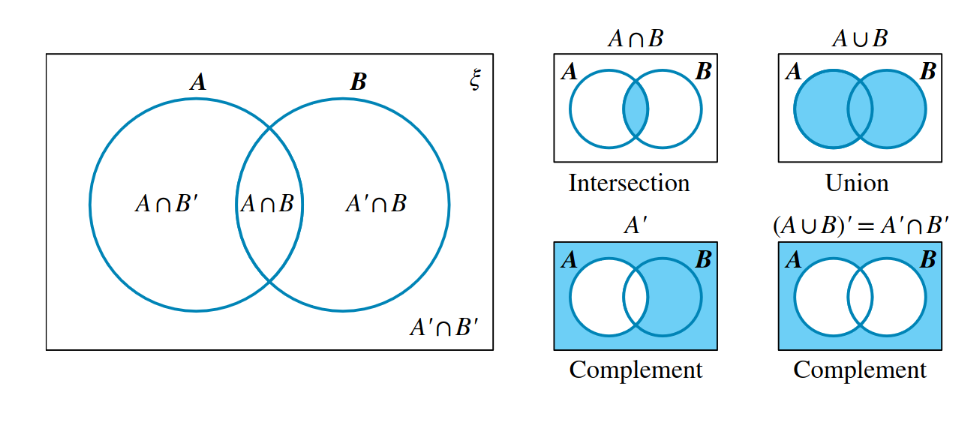
\includegraphics[scale=0.5]{venn diagrams}
\end{centre}

\section{Combinations}

\section{Pascal's triangle}

\section{Geometric sequences}

\end{document}


